\chapter{Literature Review}
% \section{Themes}

% To develop the artefact and conduct thorough background research on relevant literature to further my 
% knowledge of the subject areas, key general themes of the project were identified in Table \ref{tab:themes}. From these themes, further 
% keywords to be used in the literature search were derived to ensure that retrieved literature is directly relevant 
% to my research and development of the final artefact. Due to the constantly evolving fields the project focuses 
% on, it will be necessary to limit the results to primarily those written in recent years as there are 
% frequent new developments in the subject areas.


% \begin{table}[H]
%     \centering
%     \begin{tabular}{|p{0.2\textwidth}|p{0.55\textwidth} | p{0.2\textwidth}|}
%         \hline
%         \cellcolor{blue!25}Theme & \cellcolor{blue!25}Description &
%         \cellcolor{blue!25}Keywords \\

%         \hline

%         AI & A field of computing dedicated to allowing computers to simulate human
%         learning by training them on large amounts of data so that they can recognise patterns to classify or 
%         predict unknown data. AI can only be as good as the data it is trained upon ("Garbage in, garbage out"), and could
%         become \newline biased if it is fed too much data of a certain type. & Generative AI, 
%         Human-Centred AI, Explainable AI, AI Ethics, AI Bias \\

%         % \hline

%         % Generative AI & AI dedicated to the generation of content rather than prediction or 
%         % classification. It is possible for generative AI to produce text, images and 
%         % more recently, even video and sound. & LLMs, Tokens, Embedding \\

%         \hline

%         Natural Language Processing & NLP refers to the use of machine learning to encode and 
%         process text to understand it in a similar way to humans, which can be used to allow direct 
%         two-way conversation between users and computers. & Vectorisation, Embedding models,
%         Semantic search

%         \\

%         \hline
        
%         LLMs & Large Language Models are a type of machine learning model dedicated to the recognition and generation of text.
%         As suggested by their name, they are trained on enormous amounts of text data, which allows them 
%         to have active conversations with users. There are many different LLMs, and as their size and 
%         complexity increases, so too does the necessary processing power. &
%         Fine-tuning, Prompt engineering, Impact on industry,
%         GPT4o, LLaMA, Gemini, Evaluation
        
%         \\
%         \hline 

%         Retrieval-Augmented Generation \newline (RAG) & The optimisation of the generated text output of an LLM, incorporating
%         an external data source to enhance its contextual knowledge and enhancing the subject relevancy of outputs.
%         & Embedding, Vector databases, Document retrieval, Prompt engineering\\

%         \hline
%         Chatbot \newline Conversational Agent & Software that simulates a natural conversation between the 
%         computer and end user. Many chatbots, including the one to be produced in this project, utilise recent
%         developments such as Generative AI and natural language processing (NLP) to interpret and respond to user queries.
%         \autocite{IBMChatbotDef}
%         & NLP, Digital assistant, ChatGPT, Risks, Impact on industry \\

%         \hline

%         User Experience (UX) & The end user's overall experience of using a system, such as its ease of use and 
%         whether it is enjoyable to use. In the context of this project, it will refer to the user's 
%         ability to smoothly converse with the chatbot and how human-like it is. 
%         & Conversational design, usability, accessibility, human-computer interaction

%         \\

%         \hline 

%     \end{tabular}
%     \caption{The themes and keywords used in the literature search.}
%     \label{tab:themes}
% \end{table}


% \pagebreak % REMOVE IF NECESSARY

\section{Review of Literature}

\subsection{Artificial Intelligence (AI)}

Researchers have always wanted to harness the processing power of computers to act in a manner 
indistinguishable from that of humans from as long ago as 1950, where the question was posed 
'Can machines think?' \autocite{turing_icomputing_1950}. Ever since, constant innovations were made in computer 
intelligence and machine learning, from playing games of checkers at a better level than human players \autocite{samuel_studies_1959}
to classifying the contents of millions of images using convolutional neural networks \autocite{krizhevsky_imagenet_2012}.

Recently, AI is used across many disciplines for different purposes to complete tasks faster than, and in some cases better than,
human workers, especially with the introduction of large language models (LLMs) \autocite{AIDigitalAssistants}. \textcite{wirtz_brave_2018} write that 'service robots'~\footnote{Defined as "system-based autonomous and adaptable interfaces that 
interact, communicate and deliver service to an organization’s customers" \autocite[p.909]{wirtz_brave_2018}} can complete a variety of 
tangible or intangible actions, such as two-way conversation with chatbots.

\begin{figure}[H]
    \centering
    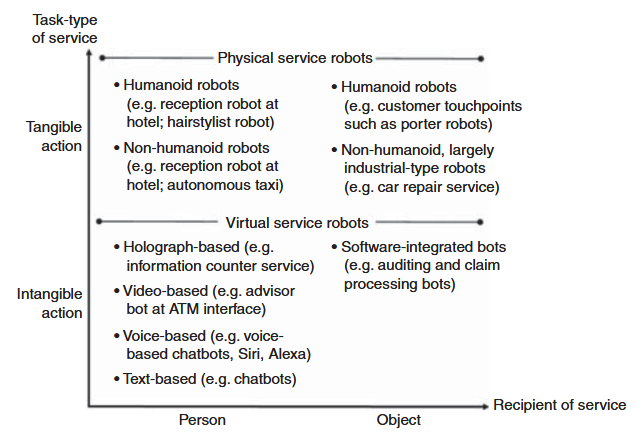
\includegraphics[width=.8\linewidth]{Literature Review/serviceBots.png}
    \caption{Service robots categorization by task-type and recipient of service \autocite{wirtz_brave_2018}.}
    \label{fig:serviceBots}
\end{figure}

When developing an AI project, it is important that the development process
is ethical and human-centred, which is known as Human-Centred AI (HCAI). 
Another issue is the "black-box problem" - the inability to know an AI's reasoning, meaning that 
eXplainable AI (XAI) is a growing necessity \autocite{miro-nicolau_comprehensive_2025}. 

Focusing on HCAI and XAI means the focus shifts from the machine to the user and their experience 
using the AI. \textcite{AIEthics} strongly advocates for the 
promotion of HCAI for the benefit of both companies and their users, which is a commonly accepted 
idea due to the ethical risks of using AI. 

Because AI calculates outcomes from its training data rather 
than understanding social norms and perspectives, using it in sociotechnical systems poses serious risks 
due to the 'traps' it can fall into, because it cannot account for every possibility such as the personal tendencies 
and biases of its users \autocite{selbst_fairness_2019}, and therefore developers require a shift in focus - from the final product
to the development process itself and end users, which also echoes Shneiderman's views. 

\subsection{Natural language processing (NLP)}
The ability for a computer to interpret and understand human language greatly enhances the scale of their capabilities. This was 
recognised during the 1950s, where machine translation from Russian to English was demonstrated for the first time, albeit in a basic form \autocite{zampolli_natural_1994}.
Ever since, NLP has been a key topic in computing, especially in recent years, with its applications widening 
in scope with modern processing power.

One of the key advancements in NLP is vectorisation, a process where data is embedded into a numerical equivalent that a computer can interpret, 
enabling Natural Language Understanding (NLU) and the identification of semantic similarities between words through the use of an embedding model 
like Word2Vec \autocite{mikolov_efficient_2013} without the need to manually label data. 
Word2Vec was a key innovation in NLP, and Mikolov and Le went on to improve it further with Doc2Vec \autocite{le_distributed_2014}, which could embed 
entire documents into semantically searchable vectorised forms.

Embedding models have further improved since, most notably with \textcite{vaswani_attention_2017}'s Transformer architecture enhancing models such as 
BERT \autocite{devlin_bert_2019}, which establishes context through analysing multiple neighbours of a word rather than reading from left to right,
gaining a higher understanding of the text it processes. Many embedding models have since been developed, though one of the most reputable is OpenAI's 
recent text-embeddings-3 model \autocite{openai_vector_nodate}, which can be used in the development of the chatbot at a low cost. 

\begin{figure}[H]
    \centering
    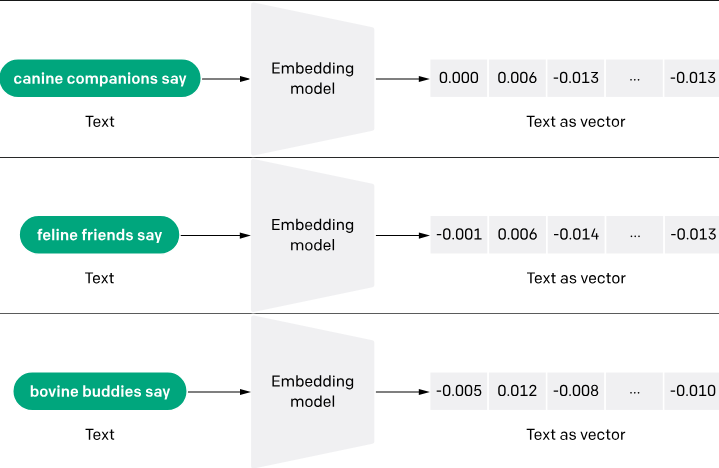
\includegraphics[width=.5\linewidth]{Literature Review/basicVectorisation.png}
    \caption{A basic overview of vectorisation \autocite{openai_introducing_nodate}.}
    \label{fig:basicVectorisation}
\end{figure}


\subsection{Large language models}
LLMs are colossal machine learning models that leverage NLP to generate text, and have become widely used across 
industries in place of technical support and human resources \autocite{vrontis_artificial_2022}. The training data required for an LLM is immense, 
reaching 45 terabytes of text data for ChatGPT in 2023 \autocite{dwivedi_so_2023}. 

This data is harvested from websites and social media due to them being the largest repositories of 
opinionated text data (\textcite{dubey_llama_2024}, \textcite{wang_fine-grained_2016}). 
However, meticulous care is taken into the specific sources used to remove 
Personally Identifiable Information (PII) to minimise privacy and ethical concerns \autocite{dubey_llama_2024}.

The previously mentioned Transformer by \textcite{vaswani_attention_2017} 
became a staple in LLMs due to the major reduction in necessary processing power to produce higher-quality 
results, and it continues to underpin many LLMs today, including ChatGPT \autocite{brown_language_2020}. 
Even with these enhancements, LLMs are still extremely performance intensive,
requiring more than 8 top-range server-grade GPUs to run some of the most powerful high-parameter models like LLaMA 3.1's 405 billion parameter model \autocite{dubey_llama_2024},
and many therefore use cloud API solutions to access LLMs.

The amount of parameters in a model does not entirely account for the quality of its responses, as studied by \textcite{ouyang_training_2022}
in Figure \ref{fig:LLMPref} wherein their surveys revealed their fine-tuned LLM "InstructGPT" with over 100x less parameters than a 175 billion parameter 
GPT3 model would often give answers preferred by its human assessors, which reveals that the fine-tuning and prompt engineering of an LLM is as vitally important
to the quality of its responses as the amount of parameters.  

% Another major innovation in LLMs came in the form of Retrieval-Augmented 
% Generation (RAG), which allows LLMs to generate answers based on an additional external data source \autocite{lewis_retrieval-augmented_2021}, such as a company's own database.
% RAG therefore allows pre-trained LLMs to be attached to another data source and generate text based on that source, which can help to reduce 
% LLM "hallucinations" \autocite{lewis_retrieval-augmented_2021}, which are occurrences where the LLM will fabricate false information as though it were correct, 
% due to the fact that it can retrieve the relevant information it otherwise may not have had.

\begin{figure}[H] 
    \centering
    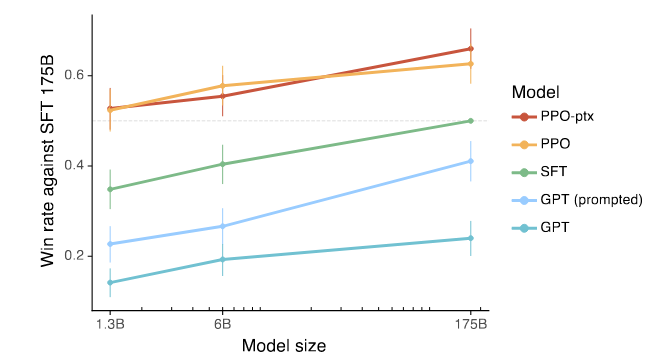
\includegraphics[width=.65\linewidth]{Literature Review/ouyangLLMPreference.png}
    \caption{Human evaluations of the GPT models produced by \textcite{ouyang_training_2022}. PPO and PPO-ptx are their models.}
    \label{fig:LLMPref}
\end{figure}

The simplest way to measure the accuracy and quality of an LLM's responses is through human evaluation surveys such as that conducted by \textcite{ouyang_training_2022}, though
software approaches such as DeepEval can be used. DeepEval offers 14 metrics to test LLM outputs with \autocite{deepeval_introduction_2024},
with a notable metric being "G-Eval", originally introduced by \textcite{liu_g-eval_2023}, which uses an "LLM-as-a-judge" approach where an LLM will evaluate
and grade the quality of the output.


\subsection{Retrieval-Augmented Generation}\label{sec:LitReviewRAG}

While LLMs are highly useful tools across many industries, they are not without limitations. The most notable 
of these limitations are hallucinations \autocite{lewis_retrieval-augmented_2021}, where the LLM will fabricate 
information that conflicts with user input, earlier conversation context or true facts \autocite{zhang_sirens_2023}. This occurs as a direct result of the LLM's parametric memory\footnote{Knowledge that the LLM has from its training data \autocite{siriwardhana_improving_2023}.}
being overfitted or biased, which can be counteracted through introducing an external knowledge source, known as non-parametric memory (\textcite{komeili_internet-augmented_2022}, \textcite{siriwardhana_improving_2023}).

\begin{figure}[H] 
    \centering
    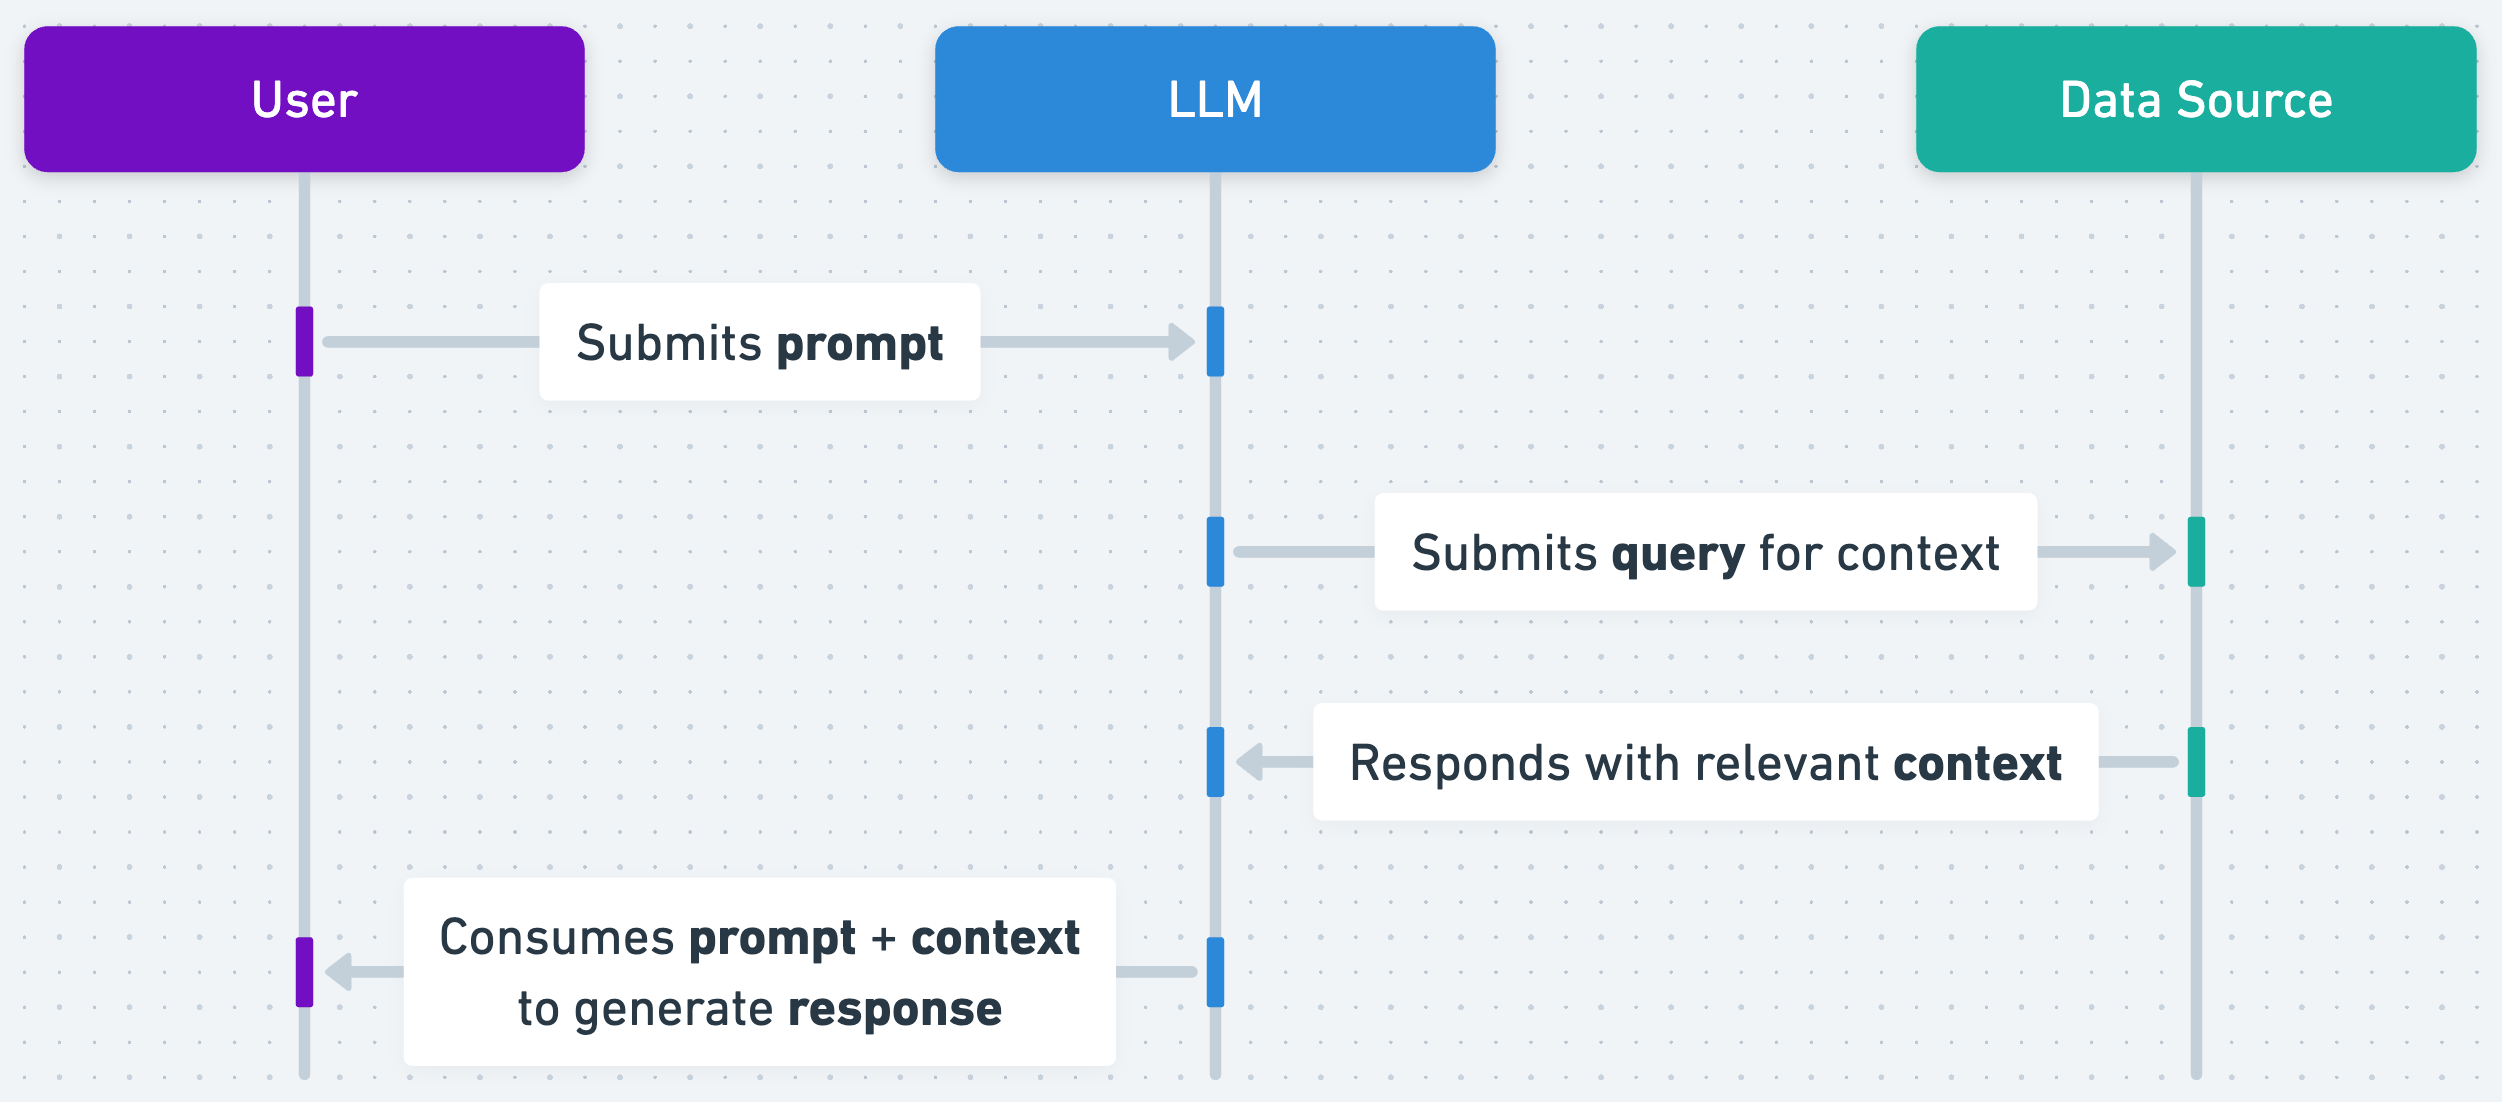
\includegraphics[width=.8\linewidth]{Literature Review/RAGProcess.png}
    \caption{A basic overview of a RAG workflow \autocite{openai_retrieval_nodate}.}
    \label{fig:RAGProcess}
\end{figure}

\textcite{siriwardhana_improving_2023} expanded upon the earlier works of \textcite{karpukhin_dense_2020} and \textcite{lewis_pre-training_2020} by creating 
"RAG-end2end", which explored the capabilities of RAG on a dynamically updating knowledge store, meaning the LLM itself would not have to be retrained 
every time the data updates, saving enormous amounts of processing power.

RAG is dependent upon external knowledge stores such as vector databases, which store and process vectorised data
for non-parametric memory \autocite{li_modernization_2023}, which makes them an essential part of the backend of 
a RAG-enabled chatbot as studied by \textcite{odede_jaybot_2024}. 

Many software options exist for
vector databases, such as Milvus \autocite{wang_milvus_2021}, Pinecone \autocite{pinecone_pinecone_nodate}, Chroma \autocite{chroma_chroma_nodate}.
\textcite{xie_brief_2023} compared these three, citing Pinecone's 'robust distributed computing capabilities and scalability', and its common usage 
in real-time searching scenarios. Pinecone was also used in chatbots by \textcite{odede_jaybot_2024} and \textcite{singer_development_2024}, showcasing its potential 
as a vector database solution for chatbots.

However, another open-source option with proven capabilities is FAISS, which was designed by engineers at Facebook (now Meta) which can be up to 8.5x faster than 
alternative options as written by \textcite{johnsonBillionscaleSimilaritySearch2017}. The speed and open-source nature of FAISS are very desirable in real-time 
applications such as chatbots, with FAISS also supporting direct integration with LLM development frameworks such as LangChain.

LangChain \autocite{langchain_introduction_nodate} is a popular open-source framework for LLM development, and RAG pipelines by extension. that can be used to connect backend elements 
together, as described by \textcite{singer_development_2024} when they used it to chunk their text data and connect to their vector database to store 
their embedded data. 


\subsection{Agentic RAG}
A very recent development in the LLM space is the use of "agents". Agents increase the capabilities of LLMs by giving them 
access to tools created by developers, effectively allowing the LLM to execute its own code to perform tasks such as web searching 
and data retrieval. Agents can also evaluate themselves, as demonstrated in Figures \ref{fig:ReActAgents} and \ref{fig:ReActRAG}, 
wherein the LLM will execute an action based on the query and evaluate the results. If the results are unsatisfactory, it can perform a slightly 
different action until a suitable answer is found. In a RAG context, this would often refer to continuous optimisation of the semantic search query 
used on the vector database.

\begin{figure}[H] 
    \centering
    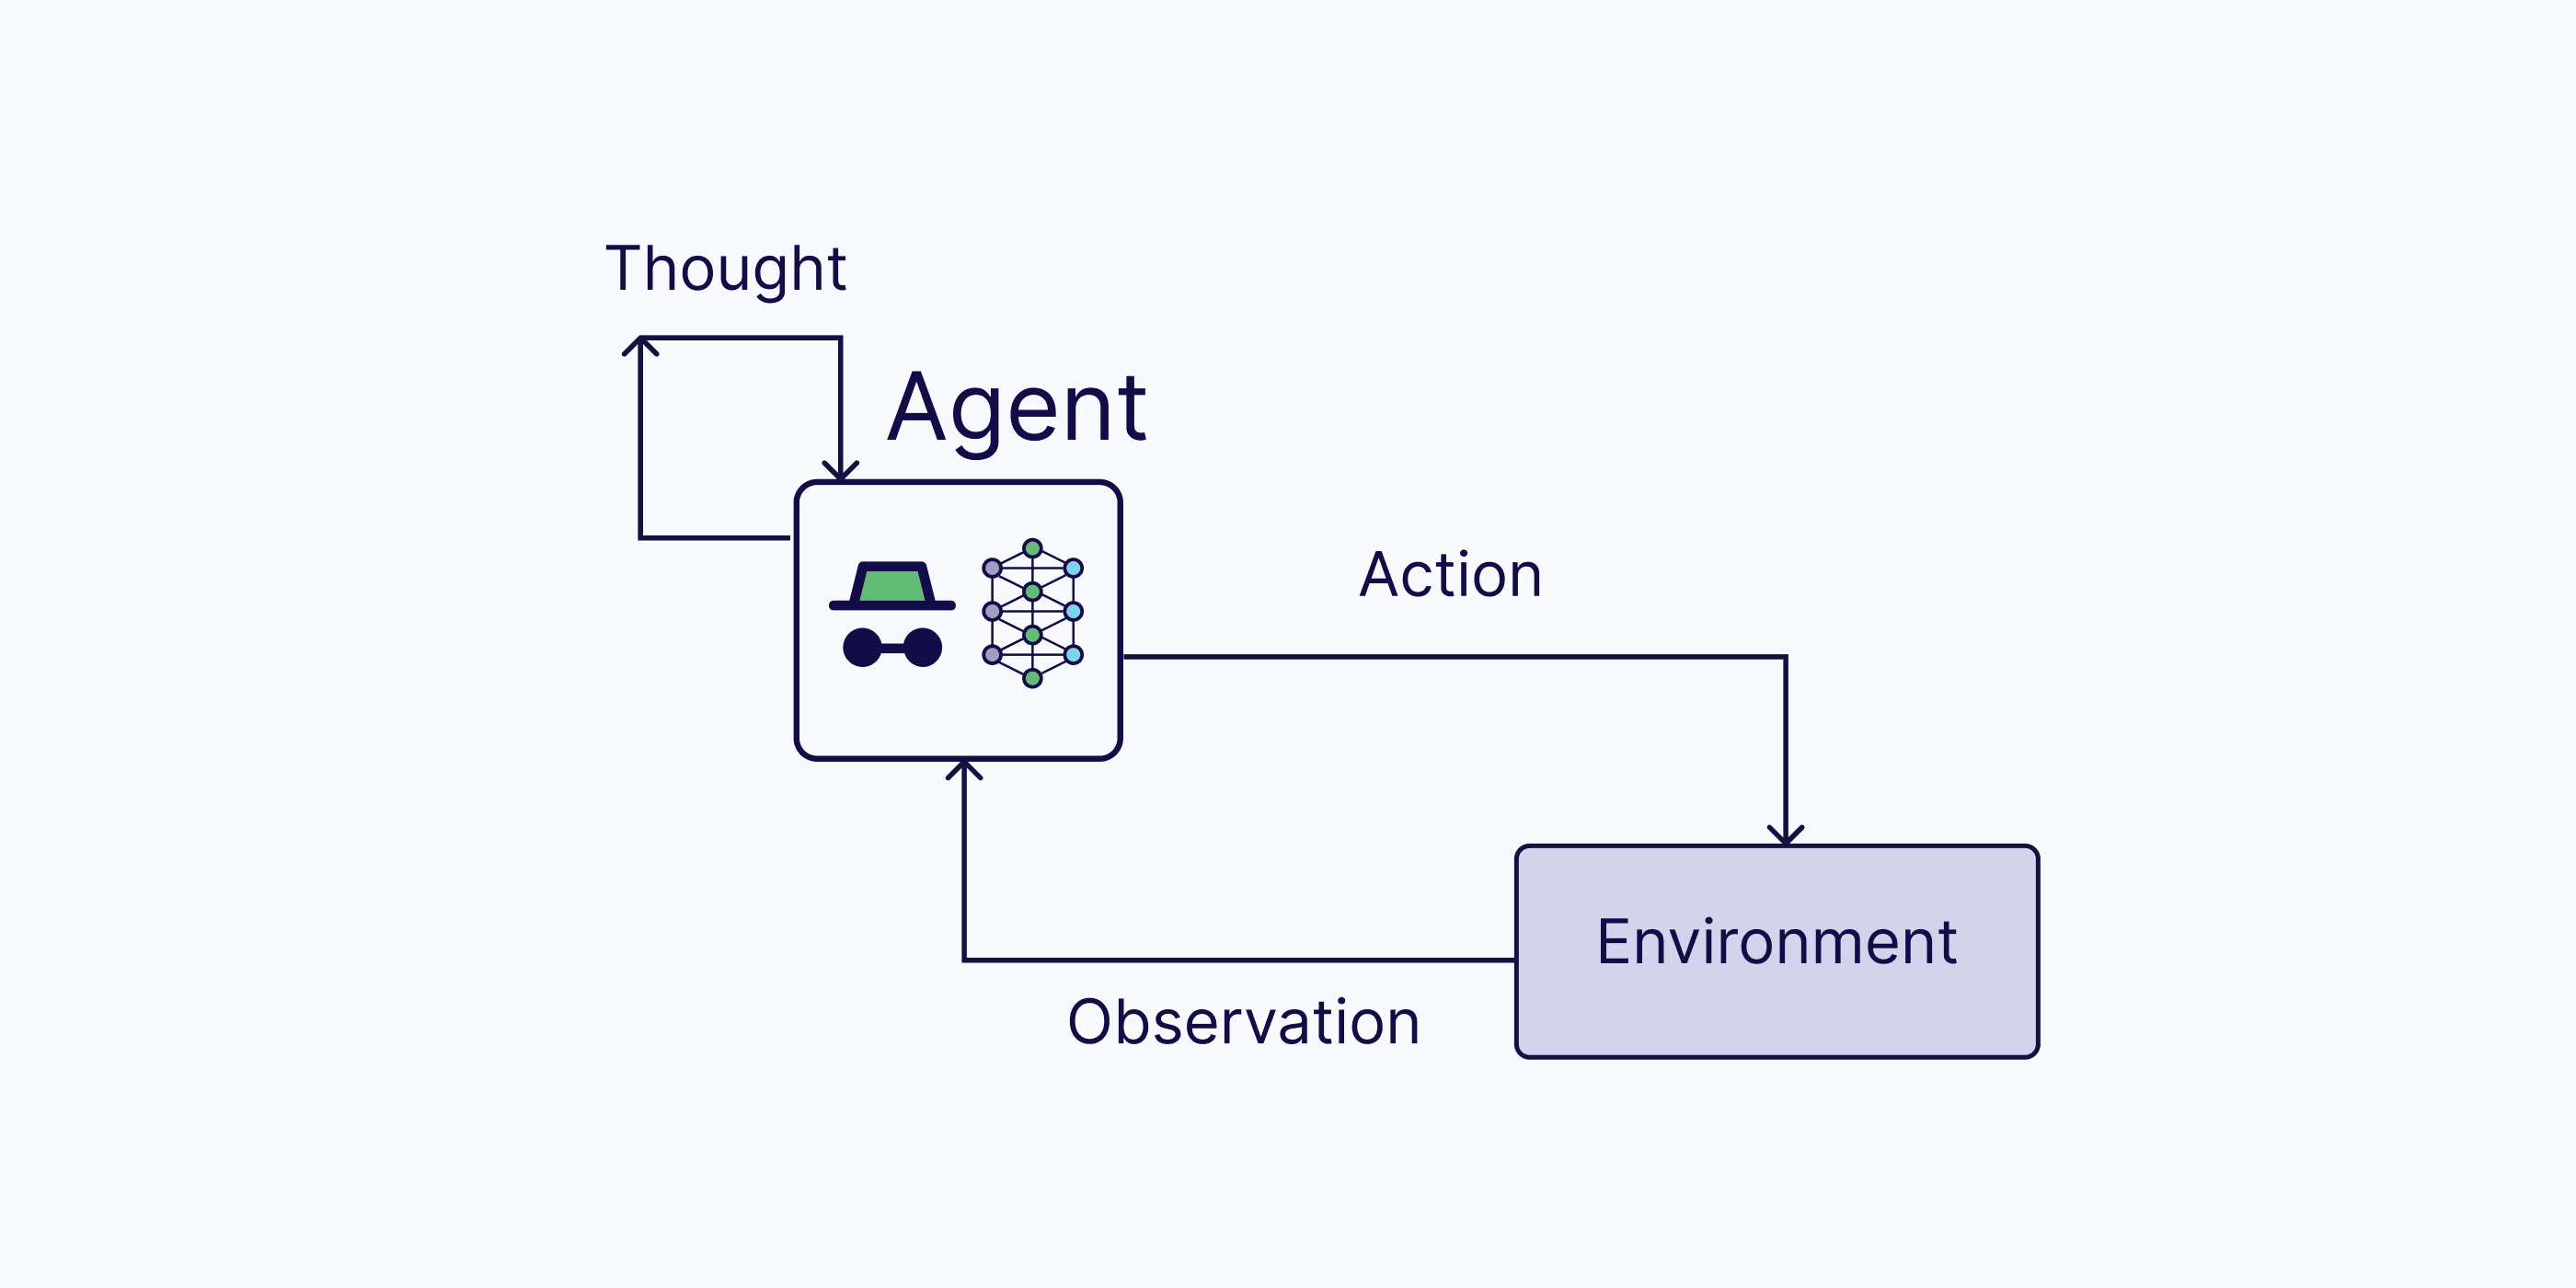
\includegraphics[width=.7\linewidth]{Literature Review/ReAct Agents.png}
    \caption{A basic ReAct (Reason + Act) agent workflow \autocite{weaviateWhatAgenticRAG2024}.}
    \label{fig:ReActAgents}
\end{figure}

\begin{figure}[H] 
    \centering
    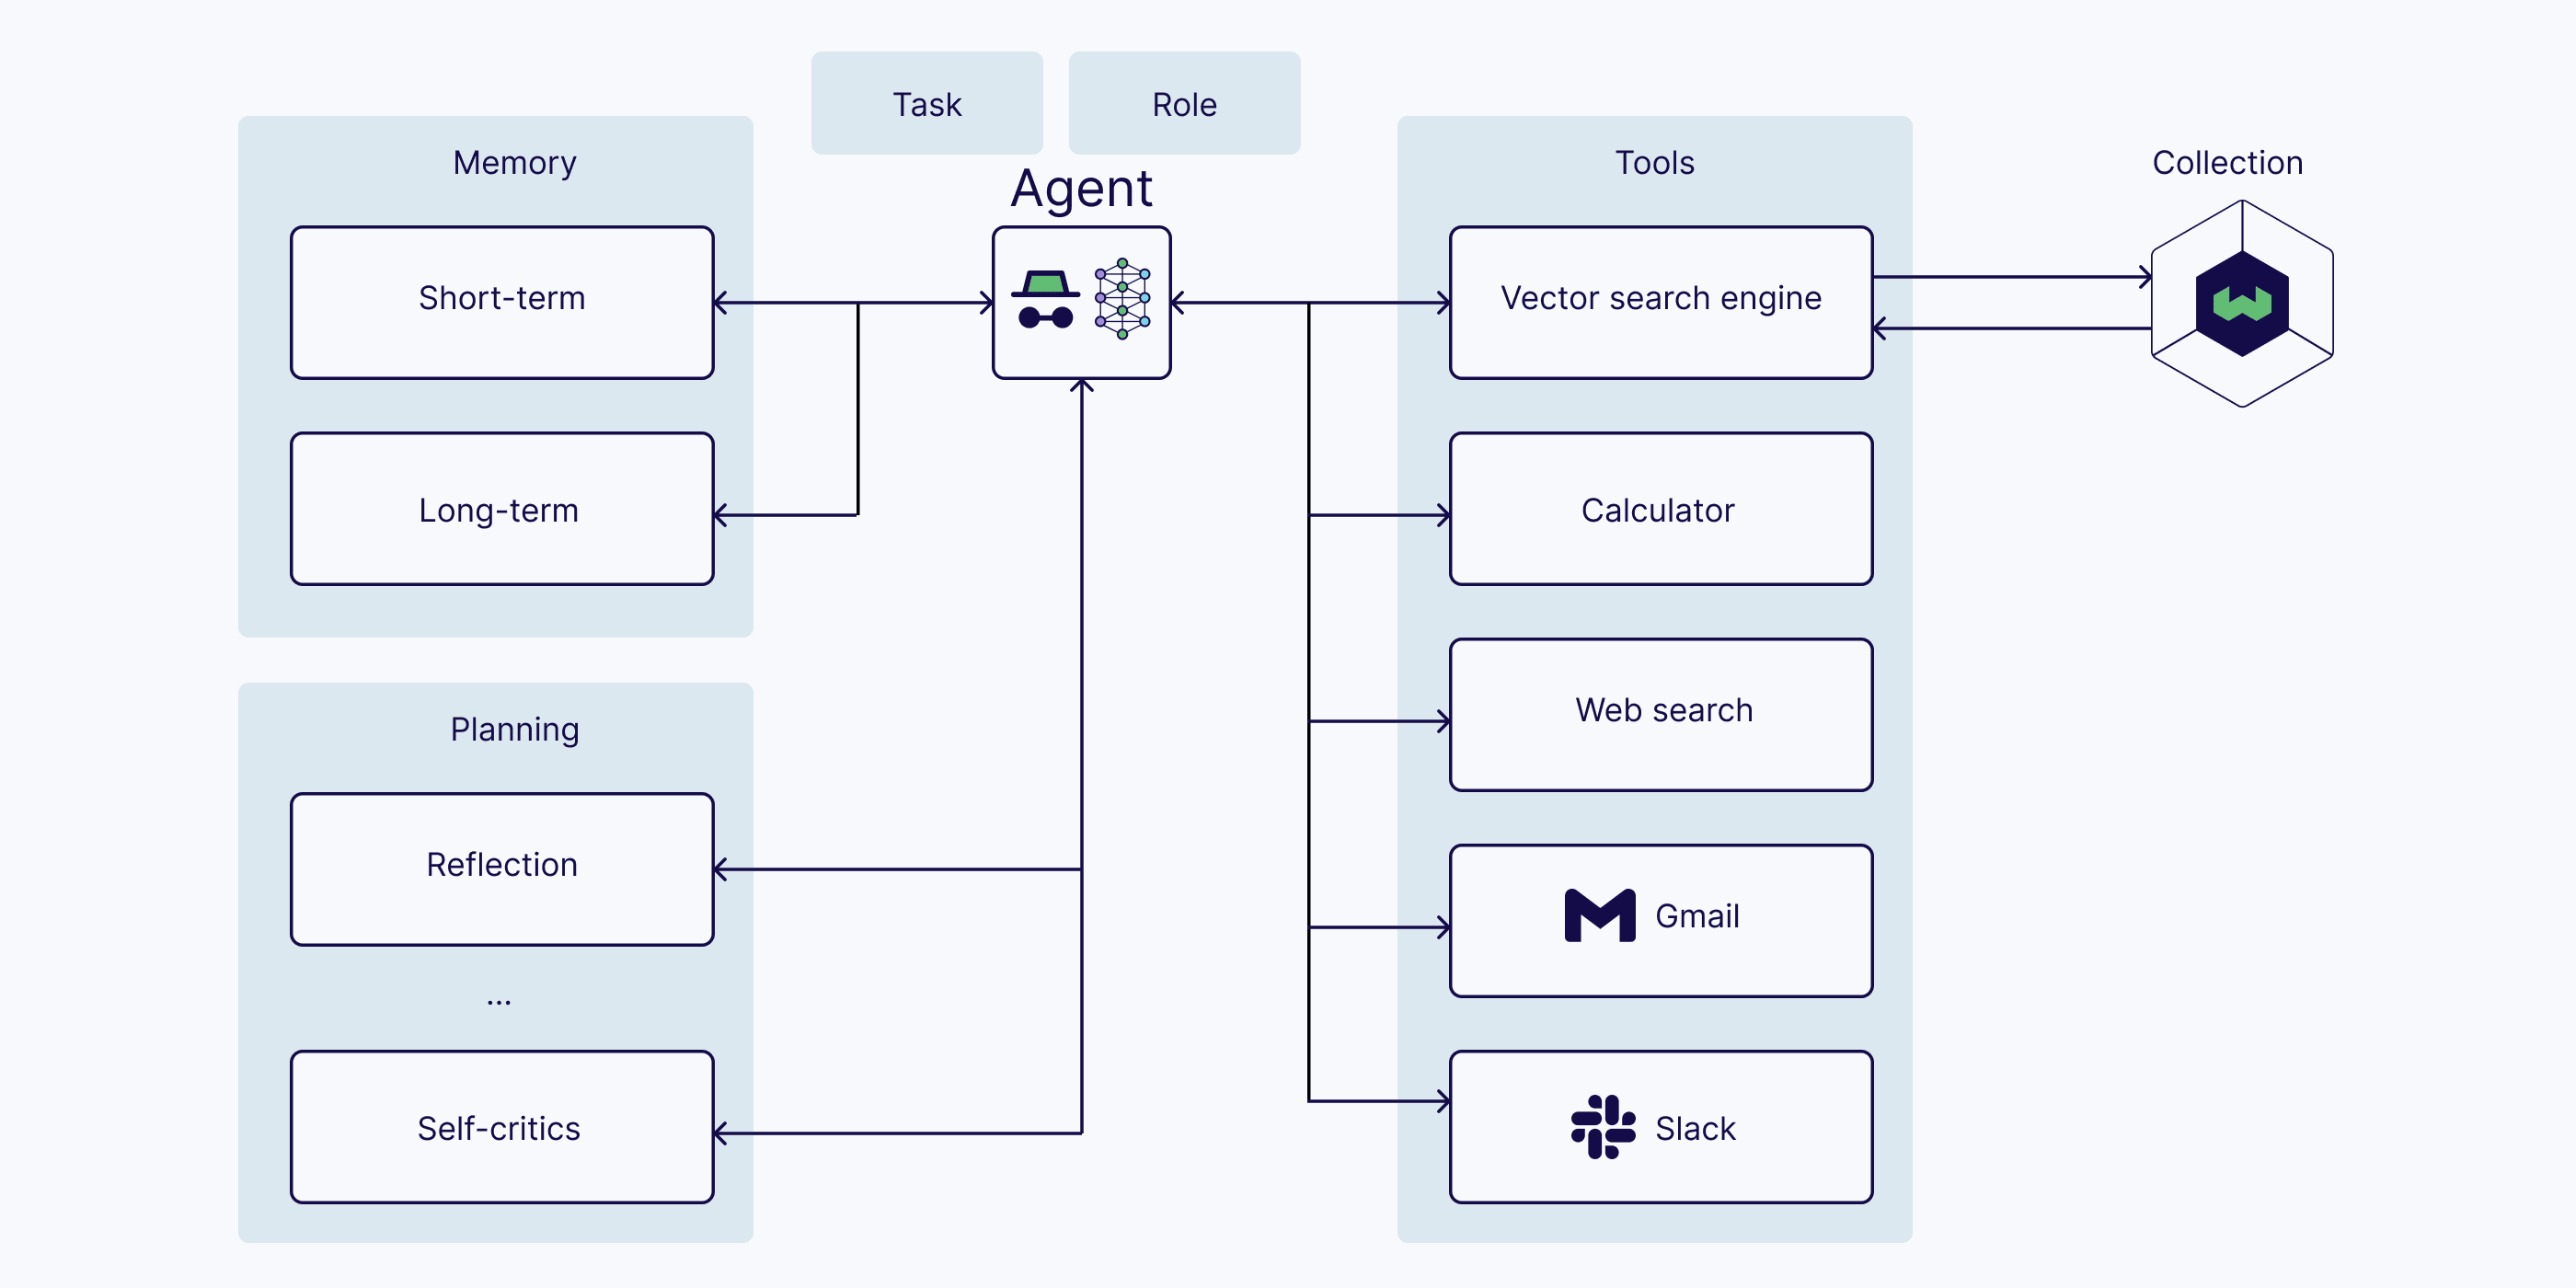
\includegraphics[width=.8\linewidth]{Literature Review/ReAct RAG.png}
    \caption{An advanced example agent workflow \autocite{weaviateWhatAgenticRAG2024}.}
    \label{fig:ReActRAG}
\end{figure}

Figure \ref{fig:ReActRAG} demonstrates the ability for agents to leverage multiple tools not only limited to searching a vector store,
and also showcases their reflective and self-evaluative capabilities. With an agent that uses an architecture like this (known as Corrective RAG/
CRAG), answers would be extensively evaluated and regenerated until the agent deems them a suitable answer to the user's query. While this largely increases the time taken to generate results, it ensures those results will be accurate and useful to the end user. 

In academic works, \textcite{wooCustomLargeLanguage2025} explored the implementation of augmenting base LLMs with agentic retrieval 
capabilities in a RAG workflow, which enhanced the accuracy of a GPT4 LLM by 95\% on their medical Q\&A dataset.

\textcite{m.branAugmentingLargeLanguage2024}'s works were among the best reviewed in demonstrating the capabilities of 
Agentic AI, with their model they named ChemCrow having the ability to call a massive variety of tools including web search 
and even accessing advanced chemistry equipment to formulate chemical catalysts from a singular natural language prompt.

\subsection{Chatbots / Conversational Agents}

Conversational agents, better known as chatbots, leverage NLP in order to simulate a conversational flow 
between a user and machine, and have become mainstream products in recent years \autocite{liao_all_2018},
though have existed as far back as 1966 with the creation of "ELIZA" for the IBM-7094 \autocite{weizenbaum_elizacomputer_1966}.
As time has passed, advancements in chatbots have occurred in "waves", where each new wave has brought a major innovation \autocite{schobel_charting_2024}.

\begin{figure}[H] 
    \centering
    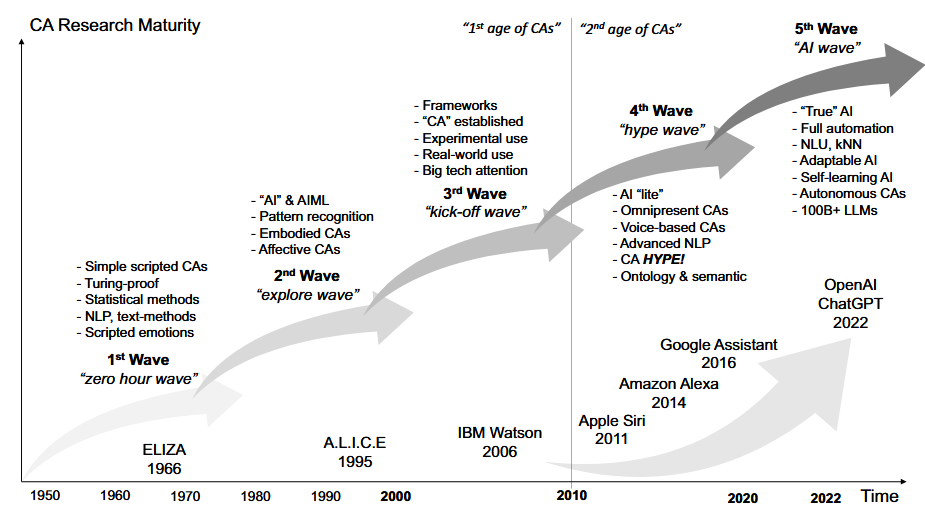
\includegraphics[width=.8\linewidth]{Literature Review/ChatbotWaves.png}
    \caption{The five waves of conversational agent research \autocite{schobel_charting_2024}.}
    \label{fig:ChatbotWaves}
\end{figure}

Due to these considerable developments in the field, chatbots are now widely used 
across industries such as education \autocite{kuhail_interacting_2023}. However, the use of the latest wave of chatbots based on LLMs
poses significant risks, especially in educational settings as studied by \textcite{neumann_llm-driven_2024},
due to the risk of hallucinations being interpreted as absolute fact, although \textcite{shuster_retrieval_2021} 
argued that this risk can be greatly reduced through introducing RAG to the backend LLM, which is further backed 
by the RAG-based chatbot created by \textcite{ge_development_2023}, which they found to also give superior answers
to those of a general-purpose chatbot without RAG.  


Many platforms exist to aid chatbot development, though they are typically aimed at users from non-IT backgrounds 
\autocite{srivastava_desirable_2020}. Popular platforms include IBM's watsonx Assistant \autocite{ibm_ibm_2024},
Google's Dialogflow \autocite{google_conversational_nodate} and Microsoft's Bot Framework \autocite{microsoft_microsoft_nodate}.
However, these are primarily targeted at enterprise clients which is reflected in their pricing. Instead of using these,
the chatbot can be manually developed using LangChain as its framework.


% \pagebreak 

\subsection{User experience and Human-Computer Interaction}

The way people interact with their devices has drastically evolved over time, from early MS-DOS command-line 
interfaces (CLIs) to mouse-based graphical user interfaces (GUIs), to touch screens \autocite{kotian_systematic_2024}, greatly broadening
the userbase of computers worldwide. Therefore, inclusive and accessible design is increasingly important to maximise the audience of any software,
especially considering the growing disabled population \autocite{putnam_how_2012}. 

As well as being inclusive, the design 
should also be user-centred, meaning it should be an iterative process that is constantly taking user feedback 
into account \autocite{chammas_closer_2015}. However, there are some barriers in this process when developing 
chatbots, as studied by \textcite{clark_what_2019} in their survey of university students who stated that they view 
chatbots as tools, and would not converse with them in the same way as they would a person, which would 
limit their potential use and hinder the overall design process. 

Users also often struggle to get chatbots to respond how they want, as their prompts may be poorly understood
due to issues like overgeneralisation \autocite{zamfirescu-pereira_why_2023}, and studies show that they
grow impatient after around 2 to 6 failed attempts, often branding the product as poor if this occurs \autocite{luger_like_2016}.

\section{Summary}
% ! Update this, it's now outdated in terms of your actual implementation and with regards to the new section.

In conclusion, this literature review has revealed multiple key focus areas for the chatbot's development. 
The overall design of the chatbot must be iterative and human-centred, and user feedback should 
be obtained at every possible opportunity to ensure the resultant product is high quality.

A deep exploration into AI, specifically in its applications in NLP, LLMs and RAG, has revealed that the best approach 
will be to leverage a pre-existing cloud-based LLM, such as GPT-4o-mini, via an API, as running an LLM on a local machine would 
require an infeasible amount of processing power.

The non-parametric memory accessed through RAG would be a vector database created with Pinecone storing embeddings generated by OpenAI's text-embeddings-3-small 
model, and the overall framework will be LangChain. This will keep the cost of the project low while maintaining a tolerable level of quality in the bot's responses.

% Invisible citing bib sources so that they'll appear in the bibliography, as they won't show up unless cited.
\nocite{IBMAIDef}
\nocite{UXDict}
\nocite{ICOAIDef}
\nocite{IBMGenAI}
\nocite{MITGenAI}
\nocite{CloudflareLLM}
\nocite{IBMNLP}
\nocite{aws_what_nodate}
\nocite{databricks_retrieval_2023}
\nocite{elastic_what_nodate}
\nocite{confident_ai_llm_nodate}
\nocite{metaFaissLibraryEfficient2017}